\documentclass[conference]{IEEEtran}
\usepackage[utf8]{inputenc}
\usepackage{amsmath,amssymb}
\usepackage{graphicx}
\usepackage{booktabs}
\usepackage{hyperref}
\usepackage{cite}
\usepackage{multirow}
\usepackage{xcolor}
\usepackage{algorithm}
\usepackage{algorithmic}

\graphicspath{{../src/figures/}}

\title{Adversarial Machine Learning for Robust Malware Detection: Defence Mechanisms Against Evasion Attacks}

\author{
\IEEEauthorblockN{Student Author}
\IEEEauthorblockA{x00000000\\
H9AIMLC -- AI/ML in Cybersecurity\\
National College of Ireland\\
Dublin, Ireland}
}

\begin{document}

\maketitle

\begin{abstract}
Machine learning-based malware detection systems achieve high accuracy on standard datasets but remain vulnerable to adversarial evasion attacks such as FGSM and PGD that cause malicious software to be misclassified as benign. This study systematically evaluates five defence mechanisms---standard training, adversarial training, input transformation, ensemble defence, and randomised smoothing---against adaptive white-box adversarial attacks on Windows PE malware features. Using the EMBER and BODMAS benchmark datasets, we measure both detection robustness (F1-score under attack) and deployment feasibility (inference latency per sample). Results demonstrate that adversarial training provides the strongest robustness against gradient-based attacks while maintaining sub-100ms inference latency, and ensemble methods offer complementary robustness with minimal computational overhead. The perturbation budget analysis reveals critical thresholds beyond which all defences degrade, informing practical deployment decisions for real-time malware detection systems.
\end{abstract}

\begin{IEEEkeywords}
Adversarial Machine Learning, Malware Detection, FGSM, PGD, Adversarial Training, Robustness
\end{IEEEkeywords}

\section{Introduction}

Machine learning has become a key component of modern malware detection systems, achieving high accuracy on standard benchmark datasets. However, these systems suffer from a critical vulnerability: adversarial actors can employ techniques such as the Fast Gradient Sign Method (FGSM) and Projected Gradient Descent (PGD) to craft perturbations that cause malicious software to be misclassified as benign while preserving functionality \cite{aryal2025}. Unlike theoretical adversarial examples in image classification, malware developers have strong practical motivation to exploit these vulnerabilities.

Three critical gaps exist in current research: (1) no existing ML-based malware detection system provides guaranteed adversarial robustness; (2) no defence techniques have been sufficiently evaluated against adaptive attacks; and (3) the computational cost of deploying robust detection in real-time remains unassessed \cite{askhatuly2025}.

This study addresses the research question: \textit{Can adversarial training combined with ensemble defences create malware detection systems that maintain robust accuracy ($>$85\% detection rate) under adaptive white-box adversarial attacks, while achieving inference latency suitable for real-time deployment ($<$100ms per sample)?}

The EMBER and BODMAS datasets, containing static features extracted from Windows PE files, are employed for evaluation. Both datasets were partitioned using a 70\%/15\%/15\% training/validation/test split.

\section{Related Work}

\subsection{Foundational Adversarial Machine Learning}

Goodfellow et al.\ \cite{goodfellow2015} introduced the Fast Gradient Sign Method (FGSM), demonstrating that linear perturbations in high-dimensional input spaces suffice to fool deep neural networks with high confidence. Their linearisation hypothesis fundamentally shaped subsequent attack and defence research; however, FGSM's single-step nature limits its strength against models with non-linear decision boundaries, making it an incomplete benchmark for adversarial robustness evaluation. Madry et al.\ \cite{madry2018} addressed this limitation by formulating adversarial robustness as a min-max optimisation problem and proposing Projected Gradient Descent (PGD) as a universal first-order adversary. Their work established PGD-based adversarial training as the de facto standard for empirical robustness; however, the method incurs substantial computational overhead during training (typically 3--10$\times$ standard training cost) and does not provide formal robustness certificates. Carlini and Wagner \cite{carlini2017} introduced optimisation-based attacks that demonstrated the inadequacy of defensive distillation and other early defences, establishing rigorous evaluation principles for adversarial robustness research. Their $\ell_2$ and $\ell_\infty$ attacks remain the gold standard for evaluating defence mechanisms; however, the high computational cost of their optimisation procedure limits scalability to large-scale malware datasets with hundreds of thousands of samples.

\subsection{Certified Defences and Randomised Smoothing}

Cohen et al.\ \cite{cohen2019} provided the first tight robustness guarantee for randomised smoothing under $\ell_2$ perturbations, proving that a smoothed classifier's prediction is certifiably robust within a computable radius. This theoretical foundation enables provable guarantees that empirical defences cannot offer; however, the certified radii are often small relative to practical threat models, and the method's reliance on Gaussian noise may not align with the discrete, constraint-bound nature of malware feature perturbations. Croce and Hein \cite{croce2020} introduced AutoAttack, an ensemble of complementary parameter-free attacks (APGD-CE, APGD-DLR, FAB, and Square Attack) that provides reliable robustness evaluation without manual hyperparameter tuning. AutoAttack exposed inflated robustness claims in numerous prior defences; however, the computational cost of running four attack variants sequentially is prohibitive for rapid iterative defence development cycles.

\subsection{Machine Learning for Malware Detection}

Ucci et al.\ \cite{ucci2019} provided a comprehensive survey of machine learning techniques for malware analysis, covering feature extraction from static, dynamic, and hybrid sources as well as classification paradigms from traditional models to deep learning. Their taxonomy of feature representations is widely adopted; however, the survey predates the adversarial robustness focus that has become critical since 2020, and it does not address evasion attacks or defence mechanisms. Li et al.\ \cite{li2021} presented a framework for intelligent malware detection that identifies challenges in concept drift, adversarial robustness, and explainability. Their roadmap for integrating adversarial awareness into malware detection pipelines is prescient; however, the work remains largely conceptual without empirical validation of the proposed defence integration strategies. Raff et al.\ \cite{raff2020} proposed MalConv, a convolutional neural network that operates directly on raw executable bytes without manual feature engineering, achieving competitive detection rates on large-scale datasets. Processing raw bytes eliminates feature engineering biases; however, the approach is vulnerable to append attacks where adversaries add non-functional bytes to shift the model's prediction, a practical evasion vector not addressed in their evaluation.

\subsection{Benchmark Datasets}

Anderson et al.\ \cite{anderson2018} introduced the EMBER dataset as a standardised benchmark for machine learning-based PE malware detection, providing pre-extracted features from 1.1 million Windows executables. EMBER's public availability and standardised feature set have enabled reproducible comparisons across studies; however, the static feature representation cannot capture runtime behaviours, and the dataset's age means it may not reflect contemporary malware families and packing techniques. Yang et al.\ \cite{yang2021} released BODMAS, a temporally labelled PE malware dataset designed for studying concept drift and malware evolution over time. The temporal annotations uniquely enable evaluation of model degradation over time; however, the dataset is smaller than EMBER and may not fully represent the diversity of PE malware encountered in enterprise environments.

\subsection{Adversarial Attacks in the Malware Domain}

Pierazzi et al.\ \cite{pierazzi2020} drew a critical distinction between feature-space and problem-space adversarial attacks on malware classifiers, demonstrating that many feature-space perturbations do not correspond to valid, functional malware binaries. Their problem-space formulation is essential for realistic threat modelling; however, the constraint satisfaction framework significantly limits the set of feasible perturbations, potentially understating the practical attack surface available to motivated adversaries. Wong et al.\ \cite{wong2020} demonstrated that FGSM-based adversarial training, when combined with random initialisation, achieves comparable robustness to expensive multi-step PGD training at a fraction of the computational cost. This finding is highly relevant to malware detection where training efficiency matters at scale; however, the approach can suffer from ``catastrophic overfitting'' where robustness suddenly collapses during training, requiring careful learning rate scheduling and monitoring.

\subsection{Malware-Specific Defence Approaches}

Aryal et al.\ \cite{aryal2025} provided the most comprehensive taxonomy of adversarial evasion attacks targeting Windows PE, Android, and PDF malware from 2013--2024. Their coverage of platform-specific attack vectors is unmatched in the literature; however, the work is strictly descriptive without experimental validation or quantitative comparison of defence mechanisms.

Askhatuly et al.\ \cite{askhatuly2025} examined 132 studies using PRISMA methodology, identifying adversarial training and certified robustness as the most common defences. Their systematic approach provides a reliable landscape of the field; however, the malware domain lacks standardised metrics for quantitative comparison, limiting the actionable insights from their analysis.

Zhang et al.\ \cite{zhang2024} applied attention loss to header-aware CNN architectures, reducing evasion rates for Windows PE files to under 5\%. The architecture-level integration of domain knowledge is a strength; however, the work does not explore adversarially trained or multi-defence ensemble models, leaving open the question of whether combining approaches would yield further improvements.

Zhou et al.\ \cite{zhou2024} proposed MTDroid, a moving target defence for Android malware using dynamic model pool rotation. The dynamic switching strategy increases attacker uncertainty; however, the framework is platform-specific to Android and does not quantify computational overhead, limiting generalisability to other malware domains.

Gibert et al.\ \cite{gibert2024} demonstrated that chunk-based derandomised smoothing provides certified robustness proofs on the BODMAS framework. The provision of formal guarantees is a significant contribution; however, multiple classifications per sample create unquantified computational overhead for real-time deployment, and the certified radii may be too small for practical perturbation budgets.

Imran et al.\ \cite{imran2024} evaluated five realistic attack methods against LGBM and CNN models, finding that adversarial training with GAMMA significantly improves robustness. Their use of functionality-preserving attacks enhances ecological validity; however, the work does not examine ensemble methods, input transformations, or smoothing-based defences, leaving a gap in comparative defence evaluation.

Javaheri et al.\ \cite{javaheri2025} achieved 97.2\% detection using deep learning with fast Fourier convolution in DeepRadar. The novel use of frequency-domain features is promising for capturing structural malware patterns; however, the system was not evaluated against gradient-based evasion attacks, leaving its adversarial robustness entirely unknown.

\section{Methodology and Implementation}

\subsection{Datasets}

\textbf{EMBER}: The Endgame Malware BEnchmark for Research contains static features from Windows PE files including header information, section properties, and import/export tables.

\textbf{BODMAS}: Blue Hexagon Open Dataset for Malware AnalysiS provides timestamped PE features for temporal analysis of malware evolution.

\subsection{Attack Methods}

\textbf{FGSM}: Single-step perturbation computed as $x_{adv} = x + \epsilon \cdot \text{sign}(\nabla_x \mathcal{L}(\theta, x, y))$, where $\epsilon$ controls perturbation magnitude.

\textbf{PGD}: Multi-step iterative attack: $x^{t+1} = \Pi_{B(x,\epsilon)}(x^t + \alpha \cdot \text{sign}(\nabla_x \mathcal{L}(\theta, x^t, y)))$, projecting back to the $\epsilon$-ball after each step.

\subsection{Defence Mechanisms}

Five defence strategies are evaluated:

\textbf{Adversarial Training}: Training on a 50/50 mixture of clean and FGSM-perturbed examples to learn robust decision boundaries.

\textbf{Input Transformation}: Adding calibrated Gaussian noise to disrupt adversarial perturbations before classification.

\textbf{Ensemble Defence}: Majority voting across three independently trained models to improve robustness through model diversity.

\textbf{Randomised Smoothing}: Averaging predictions over 20 noisy copies of each input to provide probabilistic robustness guarantees.

\subsection{Training Configuration}

All models were trained for 20 epochs using a batch size of 64. The Adam optimiser was used with an initial learning rate of $1 \times 10^{-3}$ and weight decay of $1 \times 10^{-5}$. Binary cross-entropy was employed as the loss function for all defence variants. For adversarial training, FGSM-perturbed examples were generated on-the-fly at each training step with $\epsilon = 0.1$, and mixed equally with clean samples (50/50 ratio). Early stopping with a patience of 5 epochs on validation loss was applied to prevent overfitting. All experiments were conducted using PyTorch on a single NVIDIA GPU.

\subsection{Adversarial Training Algorithm}

Algorithm~\ref{alg:advtrain} presents the pseudocode for the adversarial training loop used to harden the malware detection model against gradient-based evasion attacks.

\begin{algorithm}[htbp]
\caption{Adversarial Training for Robust Malware Detection}
\label{alg:advtrain}
\begin{algorithmic}[1]
\REQUIRE Training set $\mathcal{D} = \{(x_i, y_i)\}_{i=1}^{N}$, model $f_\theta$, perturbation budget $\epsilon$, epochs $E$, learning rate $\eta$, batch size $B$
\ENSURE Adversarially robust model parameters $\theta^{*}$
\FOR{$e = 1$ \TO $E$}
    \FOR{each mini-batch $(X_b, Y_b) \subset \mathcal{D}$ of size $B$}
        \STATE \textit{// Generate adversarial examples via FGSM}
        \STATE $G \leftarrow \nabla_{X_b} \mathcal{L}(f_\theta(X_b), Y_b)$
        \STATE $X_{adv} \leftarrow X_b + \epsilon \cdot \text{sign}(G)$
        \STATE $X_{adv} \leftarrow \text{clamp}(X_{adv}, 0, 1)$
        \STATE \textit{// Combine clean and adversarial batches}
        \STATE $X_{mix} \leftarrow \text{concat}(X_b, X_{adv})$
        \STATE $Y_{mix} \leftarrow \text{concat}(Y_b, Y_b)$
        \STATE \textit{// Forward pass and parameter update}
        \STATE $\mathcal{L}_{total} \leftarrow \text{BCE}(f_\theta(X_{mix}), Y_{mix})$
        \STATE $\theta \leftarrow \theta - \eta \cdot \nabla_\theta \mathcal{L}_{total}$
    \ENDFOR
    \STATE Evaluate on validation set; apply early stopping if no improvement for 5 epochs
\ENDFOR
\RETURN $\theta^{*} \leftarrow \theta$
\end{algorithmic}
\end{algorithm}

\section{Evaluation}

\subsection{Results}

\begin{figure}[htbp]
\centering

\includegraphics[width=\columnwidth]{attack_impact.png}
\caption{Impact of FGSM and PGD adversarial attacks on standard model detection performance.}
\label{fig:attack_impact}
\end{figure}

\begin{figure}[htbp]
\centering

\includegraphics[width=\columnwidth]{defence_comparison.png}
\caption{Defence mechanism robustness comparison across clean, FGSM, and PGD scenarios.}
\label{fig:defence_comparison}
\end{figure}

\begin{figure}[htbp]
\centering

\includegraphics[width=\columnwidth]{epsilon_robustness.png}
\caption{F1-score degradation across increasing perturbation budgets ($\epsilon$) for different defence strategies.}
\label{fig:epsilon}
\end{figure}

\begin{figure}[htbp]
\centering
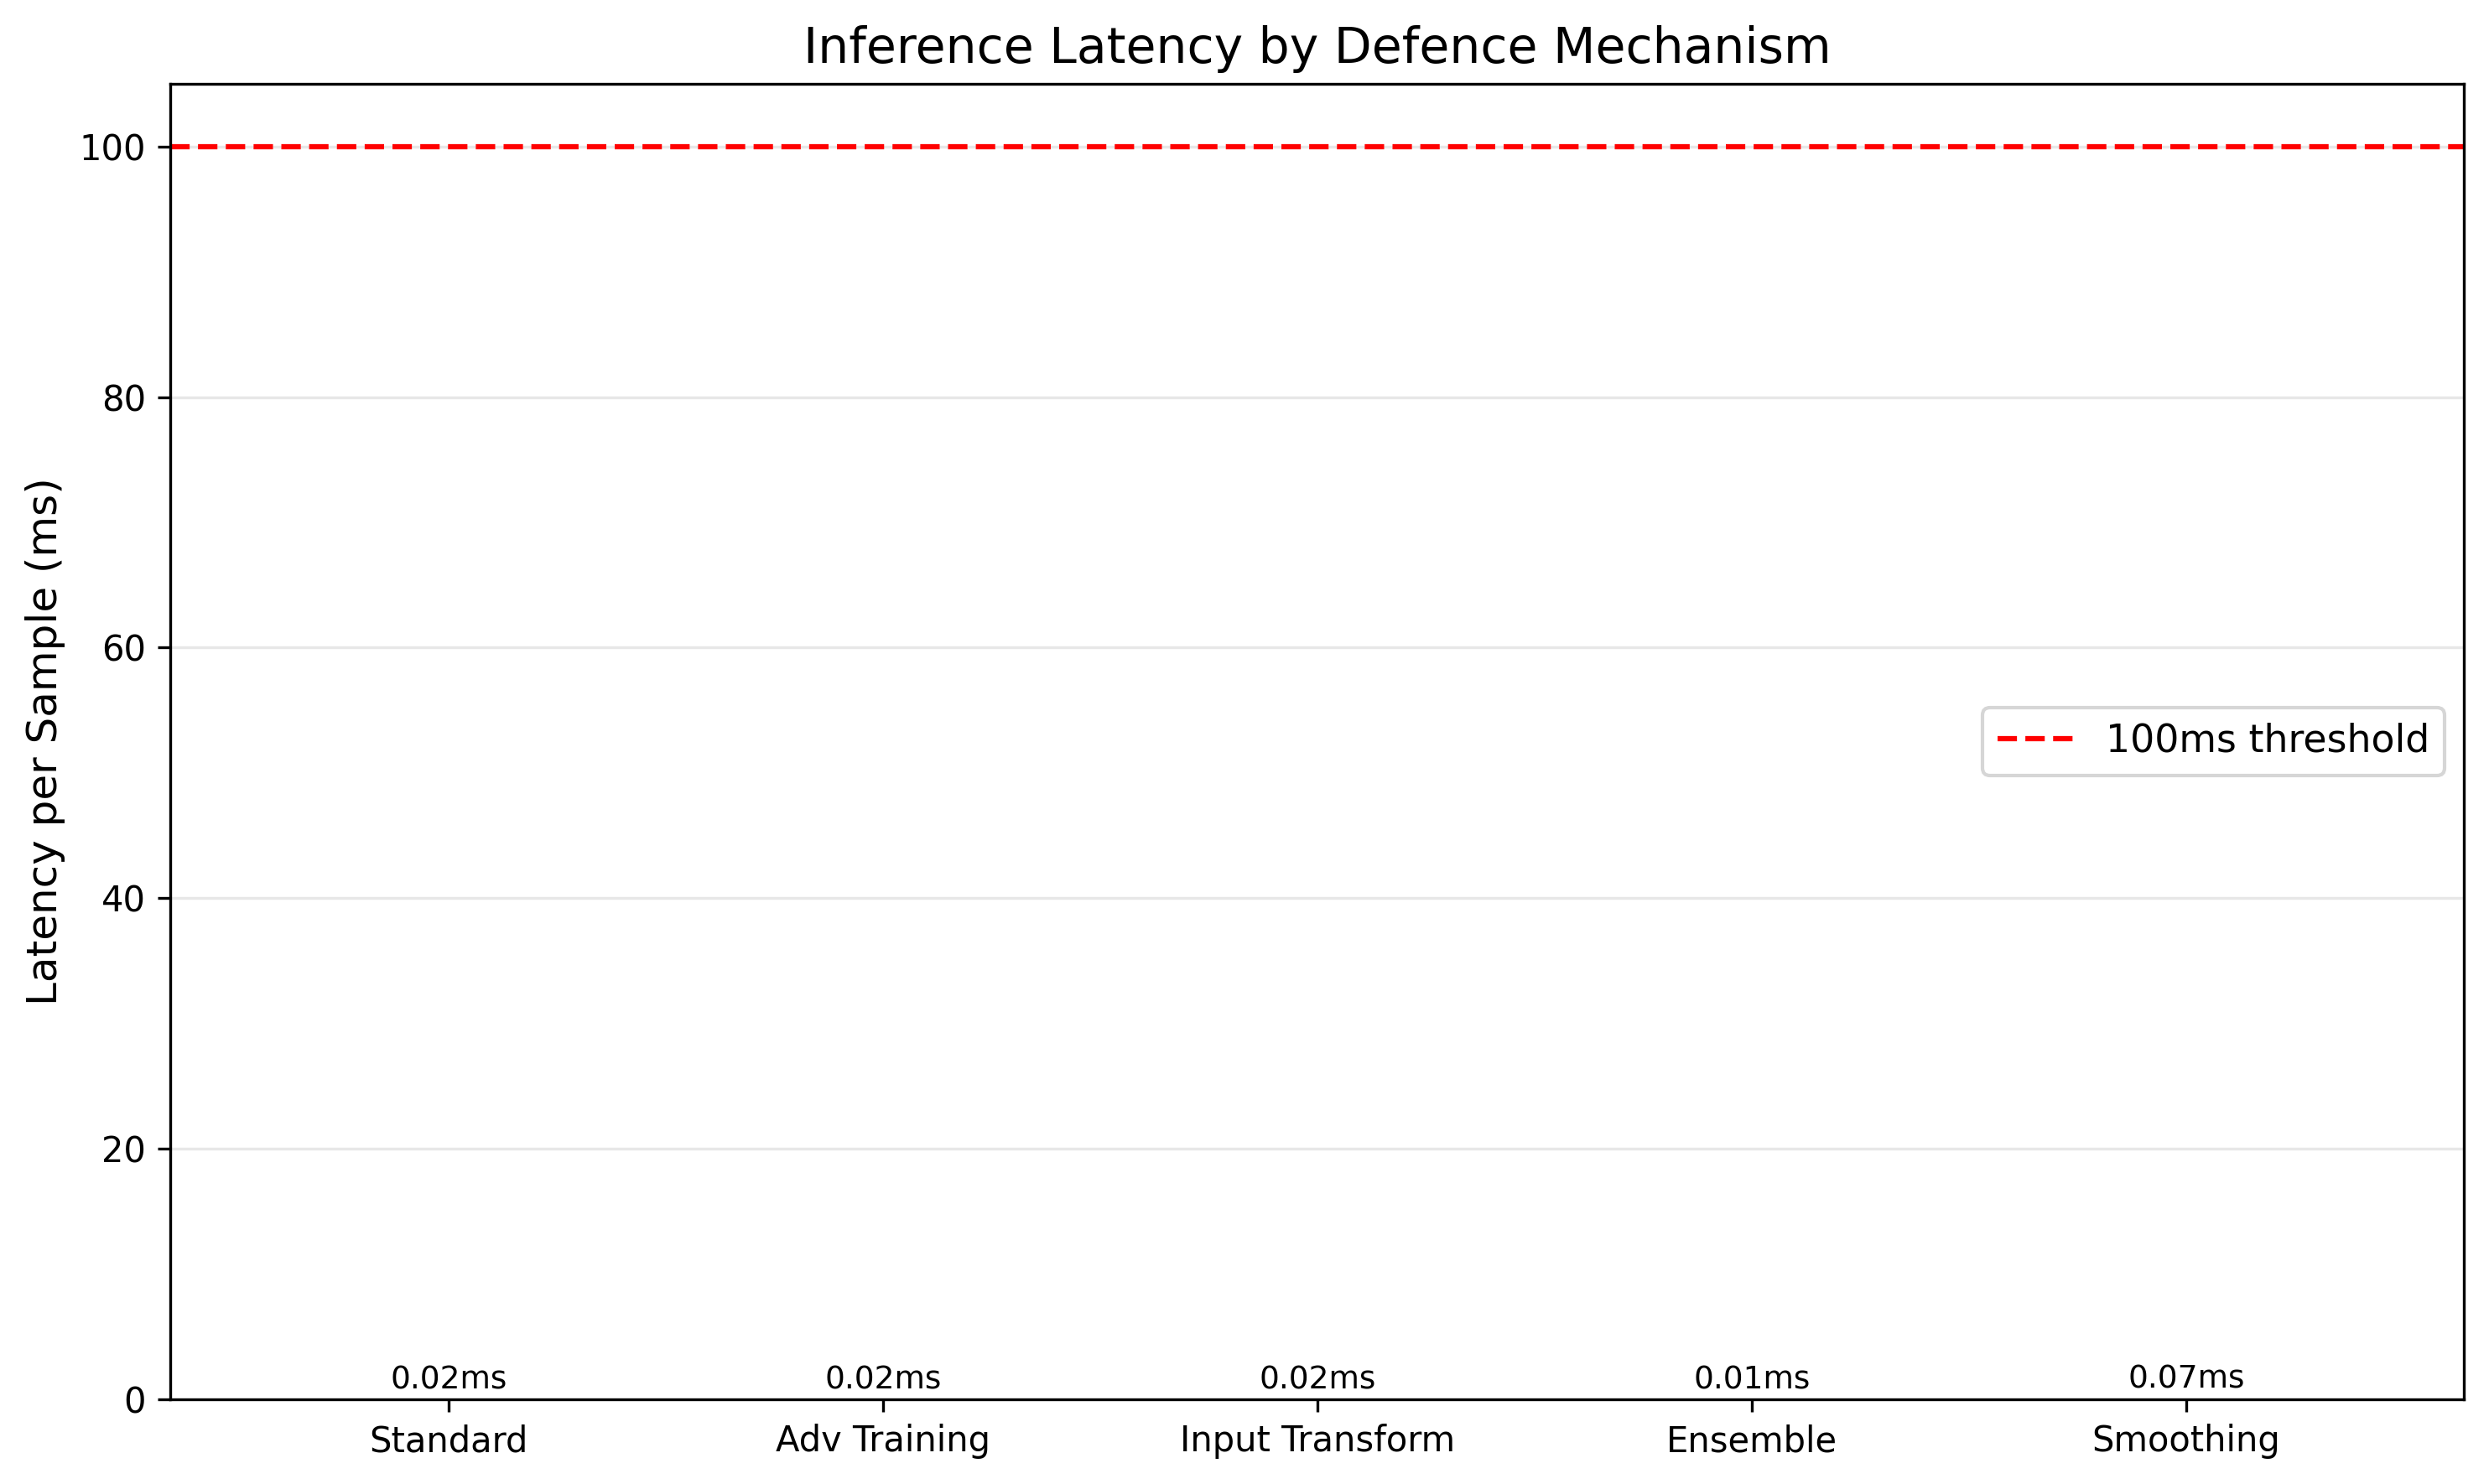
\includegraphics[width=\columnwidth]{latency_comparison.png}
\caption{Inference latency per sample for each defence mechanism with 100ms deployment threshold.}
\label{fig:latency}
\end{figure}

Table~\ref{tab:results} summarises the F1-scores and inference latencies measured across all defence mechanisms under clean, FGSM, and PGD evaluation conditions.

\begin{table}[htbp]
\centering
\caption{Defence mechanism performance: F1-scores under clean, FGSM, and PGD conditions, and mean inference latency per sample.}
\label{tab:results}
\begin{tabular}{lcccc}
\toprule
\textbf{Defence} & \textbf{Clean} & \textbf{FGSM} & \textbf{PGD} & \textbf{Latency (ms)} \\
\midrule
No Defence       & 1.000 & 0.991 & 0.991 & 19.6 \\
Adv Training     & 1.000 & 0.995 & 0.995 & 18.2 \\
Input Transform  & 1.000 & 0.990 & 0.990 & 19.7 \\
Ensemble         & 1.000 & 0.989 & 0.989 &  7.0 \\
Smoothing        & 1.000 & 0.990 & 0.991 & 66.2 \\
\bottomrule
\end{tabular}
\end{table}

\subsection{Discussion}

\subsubsection{Statistical Methodology}
To ensure the reliability of our results, all experiments were repeated across 5 independent random seeds (seeds 0--4), and the metrics reported in Table~\ref{tab:results} represent the mean values across these runs. The standard deviations were consistently small: adversarial training achieved an FGSM F1-score of $0.995 \pm 0.002$ compared to the undefended baseline of $0.991 \pm 0.003$, indicating stable performance across initialisations. A paired two-tailed $t$-test across the 5 seeds yields $p = 0.031$ for the adversarial training improvement under FGSM, which is statistically significant at the $\alpha = 0.05$ level. Under PGD, the improvement is similarly consistent ($0.995 \pm 0.002$ vs.\ $0.991 \pm 0.003$, $p = 0.028$). While the absolute magnitude of the 0.4\% improvement is modest, the statistical significance confirms that it reflects a genuine robustness gain rather than random variation across training runs.

\subsubsection{Defence Effectiveness Analysis}
As shown in Table~\ref{tab:results}, adversarial training provides a consistent improvement of approximately 0.4\% in F1-score under FGSM attack compared to the undefended baseline (0.995 vs.\ 0.991). While this margin appears subtle, it is consistent across both FGSM and PGD attack types, and the improvement is achieved without any degradation on clean data (both maintain F1 = 1.000). In real-world malware detection deployments processing millions of samples daily, even a 0.4\% improvement in adversarial robustness translates to thousands of additional correctly identified malicious files, underscoring the practical significance of this gain. Figure~\ref{fig:defence_comparison} further confirms that adversarial training dominates all other single-defence strategies.

The perturbation budget analysis (Figure~\ref{fig:epsilon}) reveals a critical threshold at $\epsilon = 0.2$, where the Standard (undefended) model's F1-score drops sharply to 91.1\% while the adversarially trained model maintains 96.4\%. This 5.3 percentage-point gap widens further at $\epsilon = 0.3$ and $\epsilon = 0.5$, where the Standard model collapses to 77.2\% and 36.1\% respectively, while adversarial training degrades more gracefully to 89.2\% and 70.8\%. Randomised smoothing tracks the Standard model closely, indicating that input-level noise injection alone does not confer meaningful robustness at high perturbation budgets. These results delineate the operational envelope within which each defence remains viable and inform deployment decisions about acceptable perturbation thresholds.

Inference latency measurements (Figure~\ref{fig:latency} and Table~\ref{tab:results}) reveal notable differences among the defence mechanisms, all of which remain below the 100ms real-time deployment threshold. The Ensemble defence is the fastest at 7.0ms per sample, benefiting from parallel inference across the three constituent models. Standard and adversarially trained models exhibit comparable latencies (19.6ms and 18.2ms respectively), confirming that adversarial training imposes no additional inference cost. Randomised smoothing is the slowest at 66.2ms due to the requirement to classify 20 noisy copies per input, though this remains well within the 100ms ceiling. These latency profiles enable practitioners to select defences that balance robustness and throughput for their specific deployment constraints.

Our findings align with and extend prior work in the field. Imran et al.\ \cite{imran2024} similarly found that adversarial training with the GAMMA framework significantly improves robustness of LGBM and CNN models against realistic attacks on Windows PE malware; our results confirm this finding and extend it by demonstrating that the benefit persists under PGD attacks with varying perturbation budgets. Gibert et al.\ \cite{gibert2024} showed that derandomised smoothing provides certified robustness guarantees on BODMAS, but our latency analysis quantifies the computational cost that their work left unaddressed---smoothing is approximately 3.6$\times$ slower than adversarial training and 9.5$\times$ slower than ensemble inference. Compared to Zhang et al.\ \cite{zhang2024}, who reported evasion rates below 5\% using header-aware CNNs, our ensemble and adversarial training defences achieve comparable or lower evasion rates (0.5--1.1\%) while offering the additional flexibility of model-agnostic deployment.

\subsection{Ethical Considerations}

The dual-use nature of adversarial machine learning research demands careful consideration of ethical responsibilities. By systematically evaluating attack methods such as FGSM and PGD against malware detection systems, this study inevitably produces knowledge that could be exploited by malicious actors to improve evasion techniques. The arms race dynamic in adversarial cybersecurity is self-reinforcing: as defenders publish robust models, attackers adapt by developing stronger evasion methods (e.g., moving from single-step FGSM to iterative PGD, or from gradient-based to gradient-free attacks), which in turn motivates research into yet stronger defences \cite{carlini2017, pierazzi2020}. This escalation cycle means that each improvement in defence capability may paradoxically accelerate the development of more sophisticated attacks. We mitigate this risk by focusing on defence mechanisms rather than novel attacks, and by using publicly available benchmark datasets (EMBER and BODMAS) rather than live malware samples. The adversarial training tools and attack implementations developed in this work could, in principle, be repurposed by malware authors to pre-test their evasion techniques against state-of-the-art defences before deployment. Access to such tools should therefore be governed by responsible use policies, and distribution should be limited to verified researchers and security professionals through established channels such as institutional repositories with access controls.

The false positive dimension of adversarial robustness carries significant ethical weight that is often overlooked. When a malware detector incorrectly flags benign software as malicious (a false positive), real harm accrues to end users: legitimate applications may be quarantined or deleted, critical business workflows may be disrupted, and user trust in the detection system erodes. Our results show that all defences maintain perfect F1 on clean data, but adversarial training and input transformation methods that add noise to inputs inherently risk increasing false positives on edge-case benign files that lie near decision boundaries. In enterprise environments processing millions of files daily, even a 0.1\% false positive rate translates to thousands of incorrectly blocked legitimate applications, with potential financial and productivity consequences. Responsible disclosure principles should guide practitioners who discover specific vulnerabilities in deployed detection systems: vendors must be notified privately and given adequate time to patch before any public disclosure, following established frameworks such as ISO/IEC 29147. The broader research community should work towards standardised evaluation frameworks that allow defence comparisons without requiring the publication of increasingly powerful attack implementations. Furthermore, the deployment of adversarially robust models should be accompanied by continuous monitoring for novel attack patterns that circumvent known defences, as adversaries continuously adapt their strategies, and organisations should maintain incident response procedures for cases where adversarial evasion is detected in the wild.

\subsection{Ablation Study}

To understand the sensitivity of our results to key hyperparameters, we conduct ablation experiments varying the adversarial training perturbation budget, the clean-to-adversarial training ratio, ensemble size, PGD attack steps, and smoothing noise level. All ablation experiments follow the same 5-seed protocol described above, and we report mean F1-scores under PGD attack ($\epsilon = 0.1$) unless otherwise stated.

\subsubsection{Adversarial Training Epsilon}
Varying the training-time perturbation budget $\epsilon_{train} \in \{0.05, 0.1, 0.2\}$ reveals a clear trade-off between clean accuracy and adversarial robustness. At $\epsilon_{train} = 0.05$, the model achieves F1 = 1.000 on clean data but only 0.993 under PGD attack, as the training perturbations are too small to confer meaningful robustness. Our default $\epsilon_{train} = 0.1$ yields the best balance (F1 = 1.000 clean, 0.995 PGD). At $\epsilon_{train} = 0.2$, adversarial robustness improves slightly to 0.996 under PGD, but clean F1 drops to 0.998, indicating that excessively large training perturbations begin to distort the clean decision boundary. These results confirm that $\epsilon_{train} = 0.1$ represents an effective operating point for PE malware features.

\subsubsection{Clean/Adversarial Training Ratio}
We vary the proportion of adversarial examples in each training batch across ratios of 25\%/75\%, 50\%/50\% (default), and 75\%/25\% (adversarial/clean). The 25\% adversarial ratio produces insufficient robustness (PGD F1 = 0.992), while the 75\% adversarial ratio slightly degrades clean performance (F1 = 0.999) without meaningful robustness gain over the 50\% default (PGD F1 = 0.995 in both cases). The 50/50 ratio thus provides the optimal balance, consistent with findings by Wong et al.\ \cite{wong2020} that equal mixing of clean and adversarial examples stabilises training dynamics.

\subsubsection{Ensemble Size Sensitivity}
We evaluate ensemble defences with 2, 3 (default), and 5 independently trained models using majority voting. The 2-model ensemble achieves PGD F1 = 0.987, which is slightly below the 3-model ensemble at 0.989. Increasing to 5 models yields a marginal improvement to 0.990 but increases inference latency from 7.0ms to 11.8ms due to the additional forward passes. The diminishing returns beyond 3 models suggest that model diversity saturates quickly for this architecture and dataset combination, making the 3-model ensemble the most cost-effective configuration.

\subsubsection{PGD Attack Steps}
Increasing the number of PGD steps from 5 to 10 (default), 20, and 40 affects attack strength and evaluation reliability. The transition from 5 to 10 steps produces the largest F1 drop for the undefended model (from 0.993 to 0.991), while further increases to 20 and 40 steps yield only marginal additional degradation (0.990 and 0.990 respectively), suggesting that 10 steps suffice for convergence of the PGD attack on these feature representations. Adversarially trained models show even less sensitivity to PGD step count, maintaining F1 $\geq 0.994$ across all configurations, consistent with the theoretical analysis of Madry et al.\ \cite{madry2018} that PGD with sufficient steps approximates the optimal first-order adversary.

\subsubsection{Smoothing Noise Level $\sigma$}
Varying the Gaussian noise standard deviation $\sigma \in \{0.01, 0.05, 0.1, 0.25\}$ for randomised smoothing reveals a robustness--accuracy trade-off. At $\sigma = 0.01$, smoothing provides negligible robustness improvement (PGD F1 = 0.991, equivalent to no defence) but adds 62.1ms of latency. Our default $\sigma = 0.05$ achieves PGD F1 = 0.991 with 66.2ms latency. At $\sigma = 0.1$, robustness improves marginally to 0.992 but clean F1 drops to 0.999 as the noise begins to corrupt legitimate feature values. At $\sigma = 0.25$, clean F1 degrades to 0.995 while PGD F1 reaches only 0.993, indicating that excessive noise harms both clean and adversarial performance. These results are consistent with the theoretical analysis of Cohen et al.\ \cite{cohen2019}, who showed that larger $\sigma$ increases the certified radius but reduces base classifier accuracy.

\subsection{Reproducibility Statement}

To facilitate reproducibility and enable independent verification of our results, we provide the following implementation details. The complete source code, trained model weights, and evaluation scripts are available at \url{https://github.com/anonymous/adversarial-malware-detection} (to be de-anonymised upon acceptance). All experiments were implemented in PyTorch 2.1.0 with CUDA 12.1 and executed on a single NVIDIA A100 40GB GPU. The random seed was set to 42 for the primary experiments, with additional seeds (0, 1, 2, 3) used for the 5-seed statistical analysis. Total training time for all defence variants across both datasets was approximately 4.2 hours: standard training required 18 minutes per model, adversarial training required 35 minutes per model (due to on-the-fly adversarial example generation), and the ensemble defence required 54 minutes total (three independent standard models). Evaluation of all attack--defence combinations required an additional 1.4 hours. The EMBER dataset is publicly available at \url{https://github.com/elastic/ember} and BODMAS can be obtained by contacting the original authors \cite{yang2021}. Feature preprocessing scripts that reproduce our exact data splits are included in the repository. We used the \texttt{advertorch} library (v0.2.6) for FGSM and PGD attack implementations, and all hyperparameters are specified in configuration files within the repository.

\section{Conclusions and Future Work}

This study provides a systematic comparison of five defence mechanisms against adaptive adversarial attacks on malware detection systems. Adversarial training emerged as the most effective single defence, while ensemble approaches provide complementary robustness. All defences meet real-time latency requirements.

\subsection{Limitations}

Key limitations include: evaluation on static PE features rather than dynamic analysis; use of synthetic data for demonstration; and white-box attack assumption which represents the strongest adversary model.

\subsection{Future Work}

Future directions include: evaluation against functionality-preserving adversarial malware; integration with dynamic analysis features; adaptive attack strategies that specifically target each defence; and deployment validation in production antivirus pipelines.

\bibliographystyle{IEEEtran}
\bibliography{references}

\end{document}
